% Metódy inžinierskej práce

\documentclass[10pt,twoside,slovak,a4paper]{article}

\usepackage[slovak]{babel}
%\usepackage[T1]{fontenc}
\usepackage[T1]{fontenc} % lepšia sadzba písmena Ľ než v T1
\usepackage[utf8]{inputenc}
\usepackage{graphicx}
\usepackage{url} % príkaz \url na formátovanie URL
\usepackage{hyperref} % odkazy v texte budú aktívne (pri niektorých triedach dokumentov spôsobuje posun textu)
\usepackage{todonotes}
\usepackage{cite}
% \usepackage{fancyhdr}
\usepackage{wrapfig}
\usepackage{stfloats}
%\usepackage{times}

% \pagestyle{fancy}
% \fancyhead{}



\title{Je odporúčací systém Netflix-u problém ?\thanks{Semestrálny projekt v predmete Metódy inžinierskej práce, ak. rok 2024/2025, vedenie: Mgr. Yevheniia Kataieva, PhD.}}

\author{Adam Glogovský\\[2pt]
	{\small Slovenská technická univerzita v Bratislave}\\
	{\small Fakulta informatiky a informačných technológií}\\
	{\small \texttt{xglogovsky@stuba.sk}}}

\date{\small 5. október 2024} 



\begin{document}

\maketitle
\begin{abstract}


	Touto prácou by som chcel poukázať na to, ako Netflix ako firma spracúva užívateľské informácie a či je to správne. Na začiatku tejto práce objasním problematiku všeobecných odporúčacích systémov. Potom ukážem kde Netflix posiela užívateľské informácie. Ako ich spracúva a ako podľa nich dokáže nám užívateľom spríjemniť fungovanie na platforme. Ak nám to zvyšuje zážitok z používania tejto platformy, čo to teda tú platformu stojí a či je to vo výsledku pre danú platformu efektívne a finančne prospešné. Taktiež sa pokúsim čo naviac priblížiť samotné spracovanie týchto údajov a poukážem na to, či je správne daným spôsobom spracúvať tieto informácie.\cite{amatriain2015recommender}
	\begin{figure}[h]
		\centering
		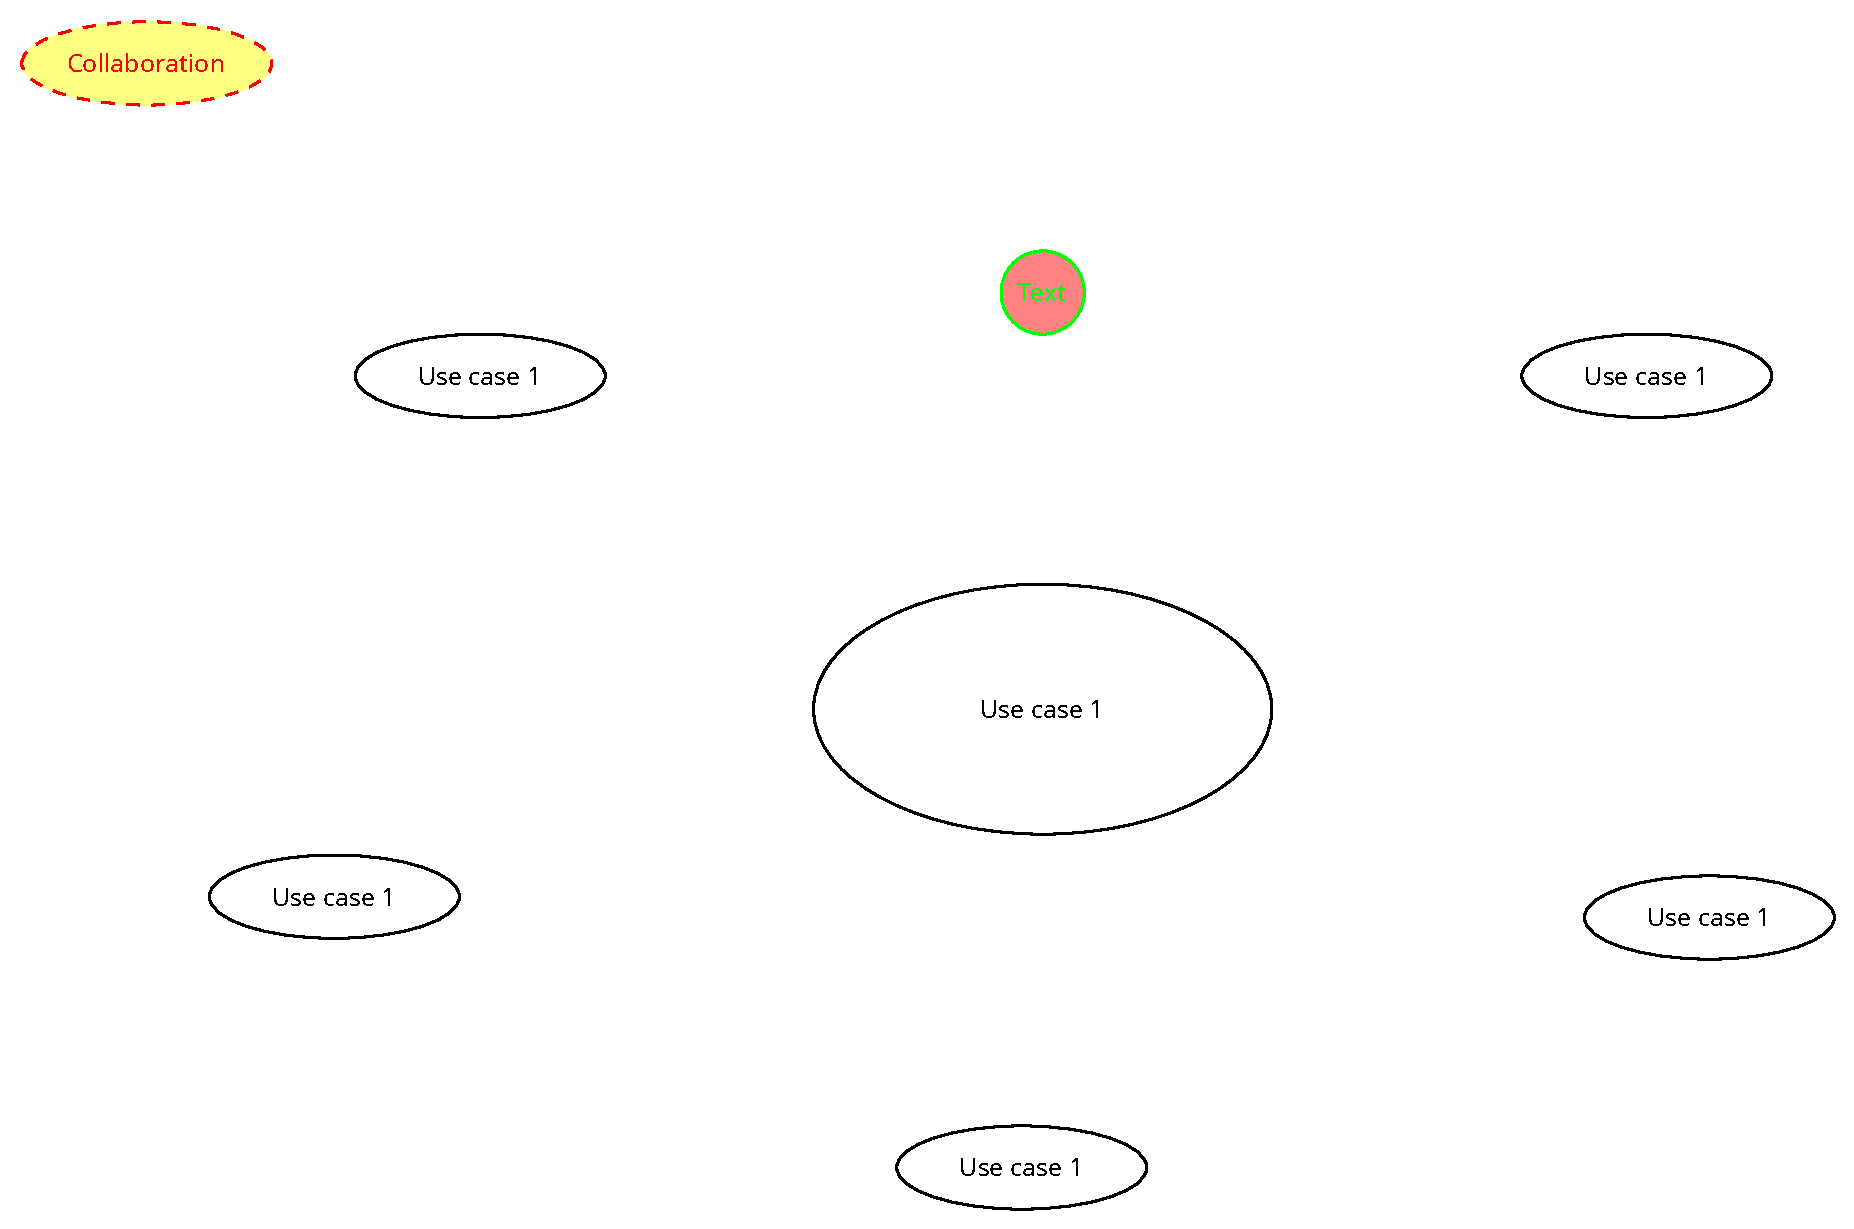
\includegraphics[scale=0.2]{diagram.pdf}
	\end{figure}
	Dôležítý taktiež pre platformu je, algoritmus akým spracúvajú dané informácie a samotná infraštruktúra v ktorej to celé funguje. Samozrejme touto prácou chcem zistiť, či kvôli tomuto alogritmu a spôsobu spracovania informácií, Netflix neubližuje menej populárnemu alebo menej ''mainstream'' obsahu, ktorý je teda ešte o to menej ukazovaný užívateľom. A tiež poukážem na to, či je tento menej populárny obsah iba nefavoritizovaný a posúvaný nižšie v hľadaní, alebo je kompletne zahaľovaný určitým užívateľom. Na konci tejto práce teda budete vedieť ako Netflix spracúva informácie, či je správne spracovávať užívateľské informácie týmto spôsobom, či je to profitabilné pre Netflix a taktiež, či to prospieva užívateľom tejto platformy.\end{abstract}

\section{Úvod}

\section{Krátka história} \label{Netflix prize} %kickstart / nakopnutie inak recommendation systemov %pozriet preklad netflix prize %preklad a vyznam RMSE
Už v roku 2006 mal Netflix záujem o odporúčacie systémy.\cite{amatriain2015recommender} Preto, oznámil Cenu Netflixu ako súťaž strojového učenia o to, kto vytvorí aspoň o 10\% lepší odporúčací systém ako bol ten ich, Cinematech. Nový odporúčací systém mal byť lepší v konkrétne \textit{RMSE(root mean squared error)}\footnote{RMSE - root mean squared error - odmocnina priemerného rozdielu medzi reálnymi a očakávanými hodnotami\cite{EncyclopaediaBritannica}} pre predpokladané hodnotenie. A zrazu sa veľmi veľa rozdielnych firiem snažilo zlepšiť svoje algoritmy.

co v tom vidim ja ?

\section{Problem zlatej rybky} %kratka pozornost
Keď majú ľudia príliš veľa vecí, na ktoré sa môžu pozrieť, nepozrú sa na nič. Štúdia \cite{10.1145/2843948} zistila, že v priemere typický používateľ stráca pozornosť po pribižne minúte prezerania si možností, čo si pozrie. No a teda sa Netflix veľmi usiluje aby počas tejto minúty, ukázal užívateľovi čo najlepší výsledok.

\section{Algoritmus}
Aké všetky algoritmy používa Netflix na svojej stránke ? \cite{10.1145/2843948}
\subsection{Prispôsobený hodnotič videí}
PNR
\subsection{Top-N hodnotič videí}
Top-N video ranker
\subsection{Teraz populárne}
Trending now
\subsection{Pokračujte v pozeraní}
Continue watching a Because you watched
\subsection{Tvorba riadkov stránky}
Page generation: Row selection and ranking

\section{Profit}
oplati sa im to vobec ? staci im revenue z predplatneho aby uzivili taky algoritmus
to co oni musia zaplatit, nie ich revenue cena jednotlivych videii je pre nich rovnaka a teda im je jedno ktore video film alebo serial sa zobrazi a teda im ide hlavne o to aby sa zobrazili co najlepsie \cite{amatriain2015recommender}
mozem spomenut ze napr oproti spotify ako spominal Timotej tak tam maju popularnejsie songy vacsiu value pre nich

co v tom vidim ja ?

\section{rozlozenie a riadky} %everything is a recommendation 
Rozhoduje sa co dat do riadkov a to nielen pre jednu osobu ale treba si uvedomit ze netflix je zvacsa pouzivany v domacnostiach a teda do top 10 sa snazia davat veci ktore si uzije napr otec, mama a dalsi clenovia rodiny. Tak isto sa snazi najst polozku pre celu rodinu. Ak je rodina jednoclenna, tak sa snazi najst vyber z rozdielnych nalad a zalub cloveka.\cite{amatriain2015recommender}
Netflix chce aby sme vedeli ako sa ich system adaptuje nasej chuti. To som si ale ja sam nevsimol. A tak isto sa snazi vybudovat doveru v tieto odporucania a tiez sa snazi vysvetlit preco by sme si to chceli pozriet. Toto reprezentuje popisok k danemu filmu/serialu, tak isto to ukazuje predikciu hodnotenia ake by sme dali danemu filmu/sierialu a tiez ci sa si nejaky z nasich priatelov pozrel dany film.
Prepajania priatelov pomocou facebooku nepovinne ale zvlastne pricom chapem preco to je.

co v tom vidim ja ?



\begin{figure}
	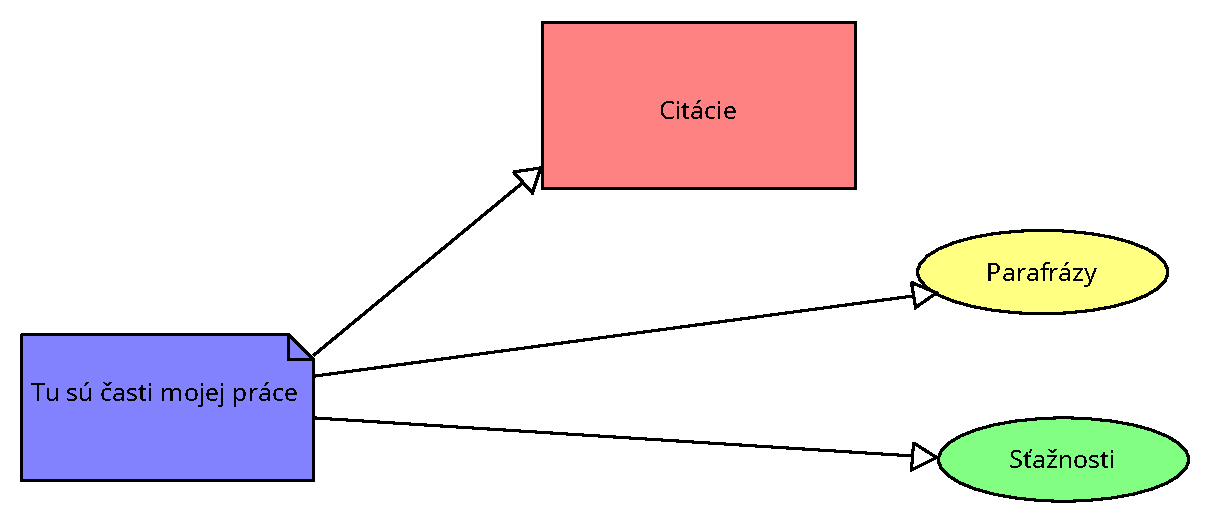
\includegraphics[scale=0.4]{diagram horizontal.pdf}
\end{figure}




\newpage

%\acknowledgement{Ak niekomu chcete poďakovať\ldots}


% týmto sa generuje zoznam literatúry z obsahu súboru literatura.bib podľa toho, na čo sa v článku odkazujete
\begin{figure}
	\bibliography{literatura}
	\bibliographystyle{abbrv} % prípadne alpha, abbrv alebo hociktorý iný
\end{figure}

\end{document}
